% =====================================================================
%  Guía de laboratorio — IEL04 — Circuitos Eléctricos I, semana 11
%  Escrita por src/guia_laboratorio.py con la plantilla institucional
%  (config/framework_iub/guia-laboratorio/: guialabiub.sty e img/, copiados a esta carpeta).
%
%  Compilar con:  pdflatex -> biber -> pdflatex -> pdflatex
%  (En Overleaf: compilador pdfLaTeX; biber se ejecuta solo.)
% =====================================================================
\documentclass[12pt]{article}

% Opciones: [sinmarca] quita la marca de agua; [borrador] muestra márgenes
%           [ieee] referencias IEEE (por defecto); [apa] referencias APA 7
\usepackage{guialabiub}

% ------- Tablas, diagramas de flujo, circuitos y gráficas (todo en LaTeX) -------
% (la plantilla no los trae; los estilos y la paleta son los del .tex del temario)
\usepackage{colortbl}                    % encabezado #121023 y filas alternas en las tablas
\usepackage{xltabular}                   % la tabla de materiales se parte entre páginas
\usepackage{tikz}
\usetikzlibrary{arrows.meta,positioning,shapes.geometric,shapes.misc}
\usepackage[siunitx,RPvoltages]{circuitikz}
\usepackage{pgfplots}
\pgfplotsset{compat=1.18}
\usepackage{adjustbox}

% Paleta del Manual de Identidad Visual IUB 2025 (los colores del manual y sus tintes)
\definecolor{iubnavy}{HTML}{121023}
\definecolor{iubyellow}{HTML}{FFDF2D}
\definecolor{iubwhite}{HTML}{FFFFFF}
\definecolor{iubblue}{HTML}{00ADE7}
\definecolor{iuborange}{HTML}{E39037}
\definecolor{iubgreen}{HTML}{3B9C6D}
\colorlet{iubgris}{iubnavy!18}
\colorlet{iubgrisoscuro}{iubnavy!60}
\colorlet{iubfondoazul}{iubblue!8}
\colorlet{iubfondonaranja}{iuborange!10}
\colorlet{iubfondoverde}{iubgreen!9}
\colorlet{iubfondogris}{iubnavy!5}
\colorlet{iubpurple}{iubnavy!45}
\pgfplotsset{cycle list={{iubblue, mark=*},{iuborange, mark=square*},{iubgreen, mark=triangle*},{iubnavy, mark=diamond*},{iubyellow, mark=pentagon*}}}

% Estilos de los diagramas de flujo (TikZ) y de las gráficas (pgfplots)
\tikzset{
  dcaja/.style={draw=iubblue, fill=iubfondoazul, line width=1pt, rounded corners=1pt, align=center, inner sep=2pt, text=iubnavy},
  destado/.style={draw=iubblue, fill=iubfondoazul, line width=1pt, rounded corners=6pt, align=center, inner sep=2pt, text=iubnavy},
  ddecision/.style={draw=iuborange, fill=iubfondonaranja, line width=1pt, diamond, aspect=1.6, align=center, inner sep=1pt, text=iubnavy},
  dterminal/.style={draw=iubgreen, fill=iubfondoverde, line width=1pt, rounded rectangle, align=center, inner sep=2pt, text=iubnavy},
  dflecha/.style={-{Stealth[length=2.4mm]}, line width=0.9pt, draw=iubnavy},
  drotulo/.style={font=\footnotesize, text=iubgrisoscuro, fill=white, fill opacity=0.92, text opacity=1, inner sep=1.5pt},
}
\pgfplotsset{iubejes/.style={width=0.9\linewidth, height=6.2cm, grid=major, grid style={iubgris}, axis lines*=left, axis line style={iubnavy}, tick label style={font=\small}, label style={font=\small}, title style={font=\bfseries\small}, legend cell align=left, legend style={draw=none, fill=none, font=\small, anchor=north, legend columns=-1, /tikz/every even column/.append style={column sep=8pt}}, unbounded coords=jump}}

% --------------------------- Bibliografía ----------------------------
\addbibresource{IEL04-semana11.bib}

% --------------------------- Datos de la guía -------------------------
\facultad{Facultad de Ingenierías}
\modulo{IEL04 --- Circuitos Eléctricos I}
\docente{Ing. Sergio Martinez Castilla}

\begin{document}

% Orden de la bibliografía: el mismo del .md (biblatex numera por orden de primera cita)
\nocite{ref1,ref2,ref3}

\datosguia
\lineablanco

% Título de la práctica y ficha de la sesión
{\centering\bfseries Guía de laboratorio: Circuito RLC en serie: tensiones antes, en y después de la resonancia y ley de voltajes de Kirchhoff\par}
\lineablanco
\textbf{Semana:} 11 de 14 \quad \textbf{Resultado de aprendizaje:} IEL04-RA4 \quad \textbf{Práctica:} propuesta a partir de la bibliografía \cite{ref1}, \cite{ref2}, \cite{ref3} \quad \textbf{Duración:} \SI{240}{\minute}
\lineablanco
La práctica corresponde a la sesión teórica de la semana 11, \guillemotleft{}El circuito RLC en serie: reactancias opuestas, ley de voltajes de Kirchhoff y resonancia en serie\guillemotright{}, y reproduce su caso de estudio: con el resistor de 100 \ensuremath{\Omega}, la bobina L3 y el condensador C2 del kit en serie, alimentados con 2,00 V eficaces, se miden la corriente y las tensiones a 3 kHz, en la resonancia y a 8 kHz, y se verifica la ley de voltajes de Kirchhoff con la bobina real. No hay un manual de laboratorio asignado al RA IEL04-RA4, por lo que la práctica se propone a partir de la bibliografía cargada: Floyd trata la impedancia, el análisis y la resonancia de los circuitos RLC en serie \cite{ref1}, Boylestad el circuito resonante en serie y el factor de calidad \cite{ref2} y Deorsola las leyes de Kirchhoff con fasores \cite{ref3}.

% ---------------------------------------------------------------------
\section{Objetivos}\label{sec:objetivos}
\textbf{Objetivo general:} Verificar experimentalmente el comportamiento de un circuito RLC en serie antes, en y después de su frecuencia de resonancia.
\lineablanco
\textbf{Objetivos específicos:}
\begin{itemize}
  \item Identificar y verificar con instrumentos el resistor, la bobina y el condensador del circuito. \emph{(CE1)}
  \item Medir la corriente y las tensiones del resistor, la bobina y el condensador a tres frecuencias. \emph{(CE2)}
  \item Localizar experimentalmente la frecuencia de resonancia del circuito RLC en serie y verificar en ella la ley de voltajes de Kirchhoff con la bobina real. \emph{(CE3)}
\end{itemize}

% ---------------------------------------------------------------------
\section{Materiales y Equipos}\label{sec:materiales}
% --- Tabla: materiales y equipos (10; xltabular repite el encabezado si se parte) ---
\arrayrulecolor{iubnavy}
\begin{xltabular}{\linewidth}{>{\raggedleft\arraybackslash}p{0.6cm} >{\raggedright\arraybackslash}X >{\raggedright\arraybackslash}X >{\raggedleft\arraybackslash}p{2.2cm}}
\caption{Materiales y equipos de la práctica}\label{tab:materiales} \\
\rowcolor{iubnavy} \textcolor{white}{\textbf{\#}} & \textcolor{white}{\textbf{Material o equipo}} & \textcolor{white}{\textbf{Especificación}} & \textcolor{white}{\textbf{Cantidad}} \\
\endfirsthead
\rowcolor{iubnavy} \textcolor{white}{\textbf{\#}} & \textcolor{white}{\textbf{Material o equipo}} & \textcolor{white}{\textbf{Especificación}} & \textcolor{white}{\textbf{Cantidad}} \\
\endhead
\bottomrule
\endlastfoot
  1 & Resistor & 100 \ensuremath{\Omega} (medido 99,5 \ensuremath{\Omega} en la sesión) & 1 \\
  \rowcolor{iubfondogris} 2 & Bobina L3 del kit & 103K, 10,4 mH y 24,6 \ensuremath{\Omega} medidos & 1 \\
  3 & Condensador C2 del kit & 104K, 97,8 nF medidos & 1 \\
  \rowcolor{iubfondogris} 4 & Generador de funciones & --- & 1 \\
  5 & Osciloscopio de dos canales con puntas \texttimes{}10 & --- & 1 \\
  \rowcolor{iubfondogris} 6 & Multímetro digital de verdadero valor eficaz & --- & 2 \\
  7 & Medidor LCR & --- & 1 \\
  \rowcolor{iubfondogris} 8 & Protoboard & --- & 1 \\
  9 & Cables de conexión & --- & 12 \\
  \rowcolor{iubfondogris} 10 & Resistencia de descarga & 1 k\ensuremath{\Omega} & 1 \\
\end{xltabular}

% ---------------------------------------------------------------------
\section{Procedimiento}\label{sec:procedimiento}
La práctica ocupa el bloque de 2 h de laboratorio de la sesión y se realiza en grupos de tres estudiantes, con tres roles que rotan entre etapas: quien monta y opera el circuito, quien mide y quien registra y verifica los cálculos. Antes de energizar cualquier montaje, el docente o el monitor revisa la conexión. Cada etapa abre con su diagrama de flujo, que muestra la secuencia y las comprobaciones de un vistazo, y sigue con sus pasos numerados; cada paso indica cuánto dura, qué debe observarse para saber que salió bien y qué hacer si no. Los valores numéricos de la sesión teórica sirven de referencia: las lecturas propias del grupo se registran en las tablas de la sección de análisis.
\lineablanco
% --- Etapa 1: Preparación y predicción (4 pasos) ---
\subsection{Preparación y predicción (\SI{32}{\minute})}\label{sec:etapa-1}
% --- Figura 1: diagrama de flujo de la etapa 1 (TikZ, con la paleta IUB) ---
\begin{figure}[H]
  \centering
\begin{adjustbox}{max width=\linewidth}
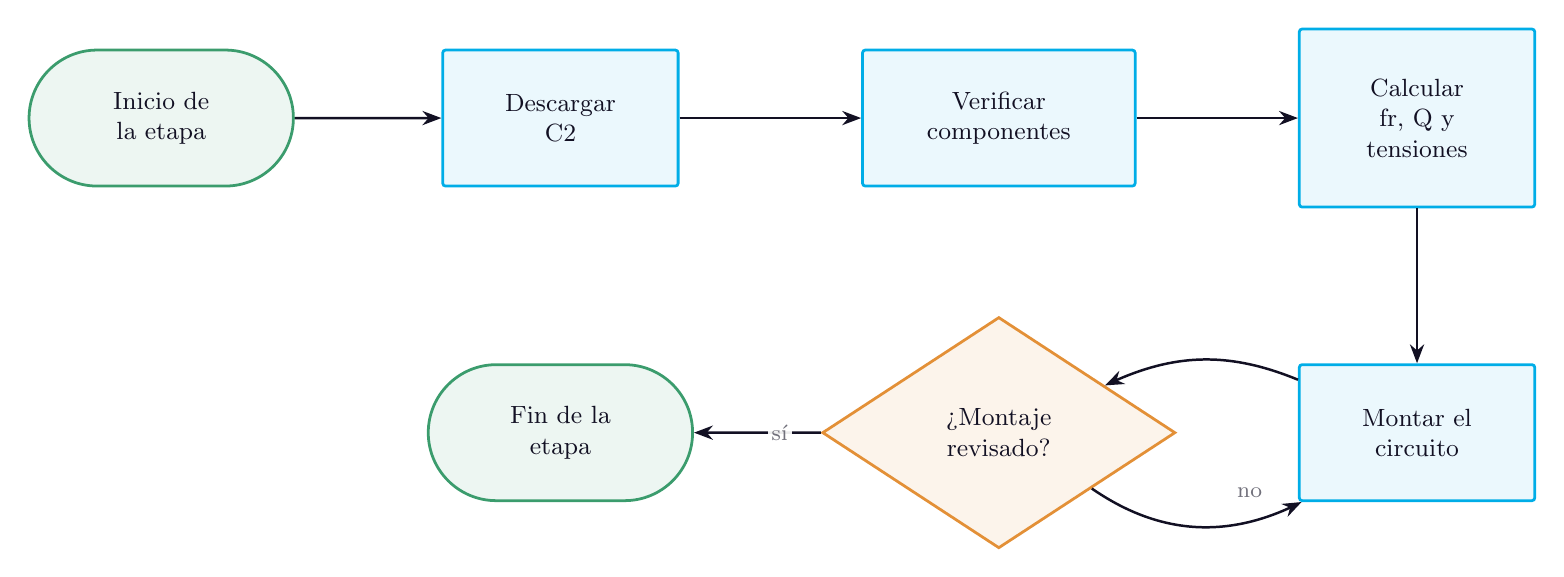
\begin{tikzpicture}[x=1in, y=1in, font=\small]
  % nodos (centro en pulgadas, con el tamano que calcula figuras.py)
  \node[dterminal, minimum width=1.377in, minimum height=0.680in] (n0) at (0.689,-0.445) {Inicio de \\ la etapa};  % ini
  \node[dcaja, minimum width=1.177in, minimum height=0.680in] (n1) at (2.685,-0.445) {Descargar \\ C2};  % a0
  \node[dcaja, minimum width=1.363in, minimum height=0.680in] (n2) at (4.877,-0.445) {Verificar \\ componentes};  % a1
  \node[dcaja, minimum width=1.177in, minimum height=0.890in] (n3) at (6.968,-0.445) {Calcular \\ fr, Q y \\ tensiones};  % a2
  \node[dcaja, minimum width=1.177in, minimum height=0.680in] (n4) at (6.968,-2.018) {Montar el \\ circuito};  % a3
  \node[ddecision, minimum width=1.766in, minimum height=1.156in] (n5) at (4.877,-2.018) {\textquestiondown{}Montaje \\ revisado?};  % dec
  \node[dterminal, minimum width=1.377in, minimum height=0.680in] (n6) at (2.685,-2.018) {Fin de la \\ etapa};  % fin
  % flechas (las de retorno, curvas)
  \draw[dflecha] (n0) -- (n1);
  \draw[dflecha] (n1) -- (n2);
  \draw[dflecha] (n2) -- (n3);
  \draw[dflecha] (n3) -- (n4);
  \draw[dflecha] (n4) to[bend right=24] (n5);
  \draw[dflecha] (n5) -- (n6);
  \draw[dflecha] (n5) to[bend right=31] (n4);
  % rotulos de las flechas (donde no caen sobre un nodo)
  \node[drotulo] at (3.781,-2.018) {sí};
  \node[drotulo] at (6.131,-2.319) {no};
\end{tikzpicture}
\end{adjustbox}
  \caption{Diagrama de flujo de la etapa 1: Preparación y predicción}
  \label{fig:flujo-1}
\end{figure}
\begin{pasos}
  \item \textbf{Paso~1:} Descargar el condensador conectando entre sus terminales, durante unos segundos, una resistencia de 1 k\ensuremath{\Omega} sujeta con pinzas aisladas, y medir con el voltímetro en cd la tensión entre terminales. \emph{(aprox.~\SI{3}{\minute})} \textbf{Comprobación:} La tensión debe ser prácticamente nula (menos de 0,1 V); si no lo es, repetir la descarga antes de manipular el componente. \textbf{Seguridad:} No cortocircuitar los terminales con los dedos ni con una herramienta metálica: un condensador puede conservar carga después de desconectado.
  \item \textbf{Paso~2:} Verificar el resistor con el ohmímetro, la bobina L3 con el medidor LCR y el ohmímetro (10,4 mH y 24,6 \ensuremath{\Omega} esperados) y el condensador C2 con el medidor LCR (97,8 nF esperados). \emph{(aprox.~\SI{8}{\minute})} \textbf{Comprobación:} Si algún valor difiere más que su tolerancia del registrado, anotar el nuevo valor y rehacer el cálculo previo con él.
  \item \textbf{Paso~3:} Calcular con los valores medidos la frecuencia de resonancia $f_r = 1/(2\pi\sqrt{LC})$, el factor de calidad $Q = X_L/(R + R_W)$ y la corriente y las tensiones esperadas a 3 kHz, en $f_r$ y a 8 kHz. \emph{(aprox.~\SI{15}{\minute})} \textbf{Comprobación:} Debe obtenerse $f_r$ cerca de 4,99 kHz y una corriente en la resonancia cerca de 16 mA.
% ecuación del paso 3: Frecuencia de resonancia y factor de calidad del RLC en serie:
\par Frecuencia de resonancia y factor de calidad del RLC en serie:
\begin{equation}
  f_r = \frac{1}{2\pi\sqrt{L C}}, \qquad Q = \frac{X_L}{R + R_W}
  \label{eq:paso-3}
\end{equation}
donde $f_r$ en Hz, $L$ en H, $C$ en F; $X_L$, $R$ y $R_W$ en \ensuremath{\Omega}; $Q$ adimensional.
  \item \textbf{Paso~4:} Montar en serie el resistor, L3 y C2, con el condensador del lado de tierra. \emph{(aprox.~\SI{6}{\minute})} \textbf{Comprobación:} El docente revisa el montaje antes de energizar. \textbf{Seguridad:} Montar con el generador apagado.
% figura del paso 4: Circuito RLC en serie con el condensador del lado de tierra (circuito en circuitikz)
\par\medskip\noindent
\begin{minipage}{\linewidth}
  \centering
  \begin{adjustbox}{max width=\linewidth}
    \begin{circuitikz}[color=iubnavy]
    \draw (0,0) to[sV, l=$v_s$] (0,3) to[R, l=$R$] (3,3) to[L, l=$L_3$] (6,3) to[C, l=$C_2$] (6,0) -- (0,0); \draw (0,0) node[ground]{};
    \end{circuitikz}
  \end{adjustbox}
  \captionof{figure}{Circuito RLC en serie con el condensador del lado de tierra}\label{fig:paso-4}
\end{minipage}
\par\medskip
\end{pasos}
% --- Etapa 2: Medición a 3 kHz y 8 kHz (3 pasos) ---
\subsection{Medición a 3 kHz y 8 kHz (\SI{26}{\minute})}\label{sec:etapa-2}
% --- Figura 3: diagrama de flujo de la etapa 2 (TikZ, con la paleta IUB) ---
\begin{figure}[H]
  \centering
\begin{adjustbox}{max width=\linewidth}
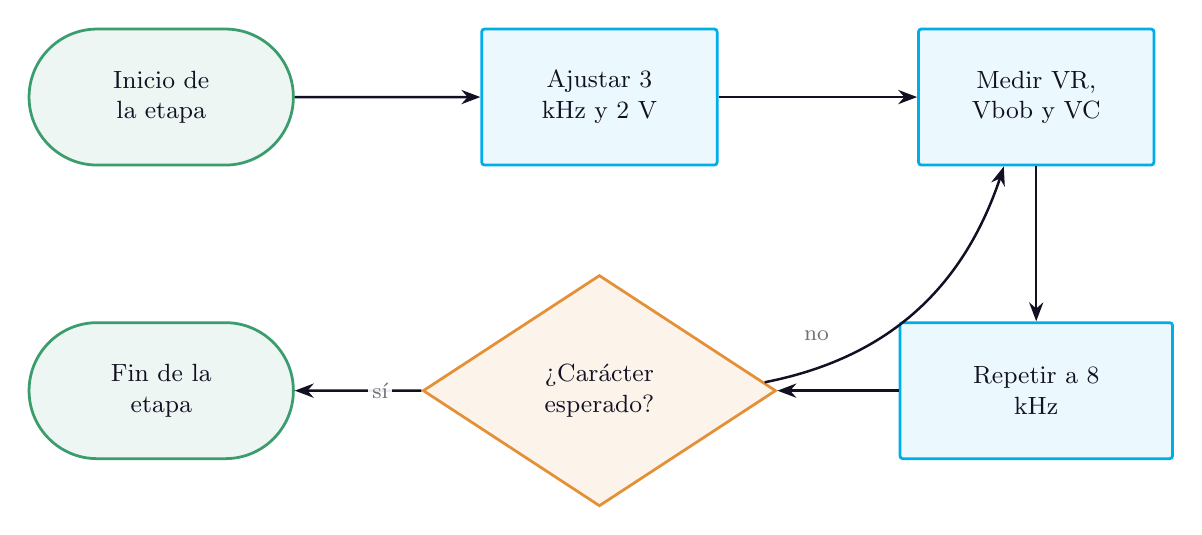
\begin{tikzpicture}[x=1in, y=1in, font=\small]
  % nodos (centro en pulgadas, con el tamano que calcula figuras.py)
  \node[dterminal, minimum width=1.377in, minimum height=0.680in] (n0) at (0.689,-0.340) {Inicio de \\ la etapa};  % ini
  \node[dcaja, minimum width=1.177in, minimum height=0.680in] (n1) at (2.880,-0.340) {Ajustar 3 \\ kHz y 2 V};  % a0
  \node[dcaja, minimum width=1.177in, minimum height=0.680in] (n2) at (5.064,-0.340) {Medir VR, \\ Vbob y VC};  % a1
  \node[dcaja, minimum width=1.363in, minimum height=0.680in] (n3) at (5.064,-1.808) {Repetir a 8 \\ kHz};  % a2
  \node[ddecision, minimum width=1.766in, minimum height=1.156in] (n4) at (2.880,-1.808) {\textquestiondown{}Carácter \\ esperado?};  % dec
  \node[dterminal, minimum width=1.377in, minimum height=0.680in] (n5) at (0.689,-1.808) {Fin de la \\ etapa};  % fin
  % flechas (las de retorno, curvas)
  \draw[dflecha] (n0) -- (n1);
  \draw[dflecha] (n1) -- (n2);
  \draw[dflecha] (n2) -- (n3);
  \draw[dflecha] (n3) -- (n4);
  \draw[dflecha] (n4) -- (n5);
  \draw[dflecha] (n4) to[bend right=31] (n2);
  % rotulos de las flechas (donde no caen sobre un nodo)
  \node[drotulo] at (1.784,-1.808) {sí};
  \node[drotulo] at (3.965,-1.535) {no};
\end{tikzpicture}
\end{adjustbox}
  \caption{Diagrama de flujo de la etapa 2: Medición a 3 kHz y 8 kHz}
  \label{fig:flujo-2}
\end{figure}
\begin{pasos}
  \item \textbf{Paso~5:} Ajustar el generador a una onda sinusoidal de 3 kHz y medir con el osciloscopio y con el multímetro de verdadero valor eficaz que la tensión en los bornes del circuito, con el circuito conectado, sea de 2,00 V eficaces. \emph{(aprox.~\SI{6}{\minute})} \textbf{Comprobación:} El multímetro debe indicar 2,00 V y el osciloscopio una sinusoide sin distorsión; si la tensión baja al conectar el circuito, reajustar la amplitud con el circuito conectado.
  \item \textbf{Paso~6:} Medir con el multímetro de verdadero valor eficaz las tensiones en el resistor, en la bobina y en el condensador, y calcular la corriente como $V_R/R$. \emph{(aprox.~\SI{10}{\minute})} \textbf{Comprobación:} A 3 kHz la tensión del condensador debe superar a la de la bobina (carácter capacitivo).
  \item \textbf{Paso~7:} Repetir a 8 kHz, reajustando la tensión de la fuente a 2,00 V eficaces. \emph{(aprox.~\SI{10}{\minute})} \textbf{Comprobación:} A 8 kHz la tensión de la bobina debe superar a la del condensador (carácter inductivo).
\end{pasos}
% --- Etapa 3: Resonancia y ley de voltajes de Kirchhoff (3 pasos) ---
\subsection{Resonancia y ley de voltajes de Kirchhoff (\SI{28}{\minute})}\label{sec:etapa-3}
% --- Figura 4: diagrama de flujo de la etapa 3 (TikZ, con la paleta IUB) ---
\begin{figure}[H]
  \centering
\begin{adjustbox}{max width=\linewidth}
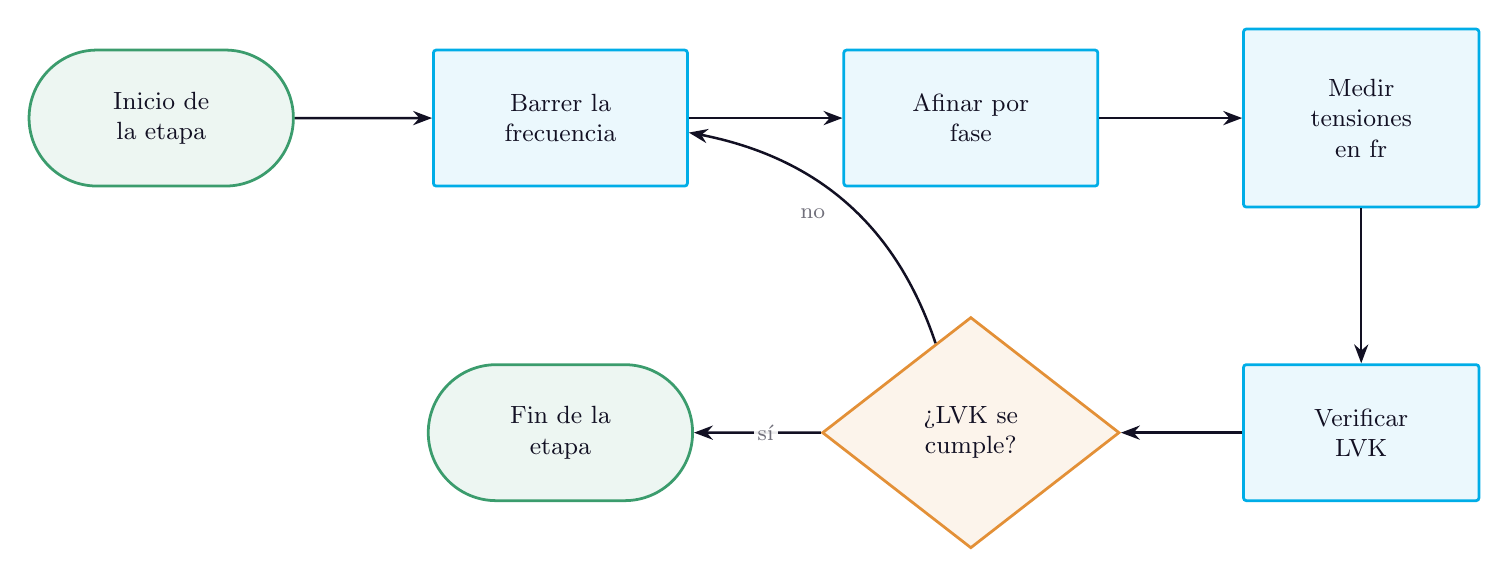
\begin{tikzpicture}[x=1in, y=1in, font=\small]
  % nodos (centro en pulgadas, con el tamano que calcula figuras.py)
  \node[dterminal, minimum width=1.377in, minimum height=0.680in] (n0) at (0.689,-0.445) {Inicio de \\ la etapa};  % ini
  \node[dcaja, minimum width=1.270in, minimum height=0.680in] (n1) at (2.685,-0.445) {Barrer la \\ frecuencia};  % a0
  \node[dcaja, minimum width=1.270in, minimum height=0.680in] (n2) at (4.737,-0.445) {Afinar por \\ fase};  % a1
  \node[dcaja, minimum width=1.177in, minimum height=0.890in] (n3) at (6.689,-0.445) {Medir \\ tensiones \\ en fr};  % a2
  \node[dcaja, minimum width=1.177in, minimum height=0.680in] (n4) at (6.689,-2.018) {Verificar \\ LVK};  % a3
  \node[ddecision, minimum width=1.487in, minimum height=1.156in] (n5) at (4.737,-2.018) {\textquestiondown{}LVK se \\ cumple?};  % dec
  \node[dterminal, minimum width=1.377in, minimum height=0.680in] (n6) at (2.685,-2.018) {Fin de la \\ etapa};  % fin
  % flechas (las de retorno, curvas)
  \draw[dflecha] (n0) -- (n1);
  \draw[dflecha] (n1) -- (n2);
  \draw[dflecha] (n2) -- (n3);
  \draw[dflecha] (n3) -- (n4);
  \draw[dflecha] (n4) -- (n5);
  \draw[dflecha] (n5) -- (n6);
  \draw[dflecha] (n5) to[bend right=31] (n1);
  % rotulos de las flechas (donde no caen sobre un nodo)
  \node[drotulo] at (3.711,-2.018) {sí};
  \node[drotulo] at (3.947,-0.924) {no};
\end{tikzpicture}
\end{adjustbox}
  \caption{Diagrama de flujo de la etapa 3: Resonancia y ley de voltajes de Kirchhoff}
  \label{fig:flujo-3}
\end{figure}
\begin{pasos}
  \item \textbf{Paso~8:} Barrer la frecuencia entre 3 kHz y 8 kHz buscando el máximo de la tensión en el resistor, reajustando la fuente a 2,00 V eficaces. \emph{(aprox.~\SI{10}{\minute})} \textbf{Comprobación:} El máximo debe aparecer cerca de 5 kHz; si no se encuentra, revisar las conexiones de la serie.
  \item \textbf{Paso~9:} Afinar la resonancia con el osciloscopio, buscando que la tensión del resistor quede en fase con la de la fuente, y anotar la frecuencia. \emph{(aprox.~\SI{8}{\minute})} \textbf{Comprobación:} La diferencia con $f_r$ calculada debe ser de pocos por ciento.
  \item \textbf{Paso~10:} Medir en la resonancia las tensiones en el resistor, la bobina y el condensador, y comprobar que $V_S \approx V_R + I R_W$. \emph{(aprox.~\SI{10}{\minute})} \textbf{Comprobación:} La tensión del resistor debe ser cercana a 1,60 V y la suma con la caída en la resistencia de devanado, cercana a 2,00 V.
\end{pasos}
% --- Etapa 4: Desmontaje y cierre (3 pasos) ---
\subsection{Desmontaje y cierre (\SI{10}{\minute})}\label{sec:etapa-4}
% --- Figura 5: diagrama de flujo de la etapa 4 (TikZ, con la paleta IUB) ---
\begin{figure}[H]
  \centering
\begin{adjustbox}{max width=\linewidth}
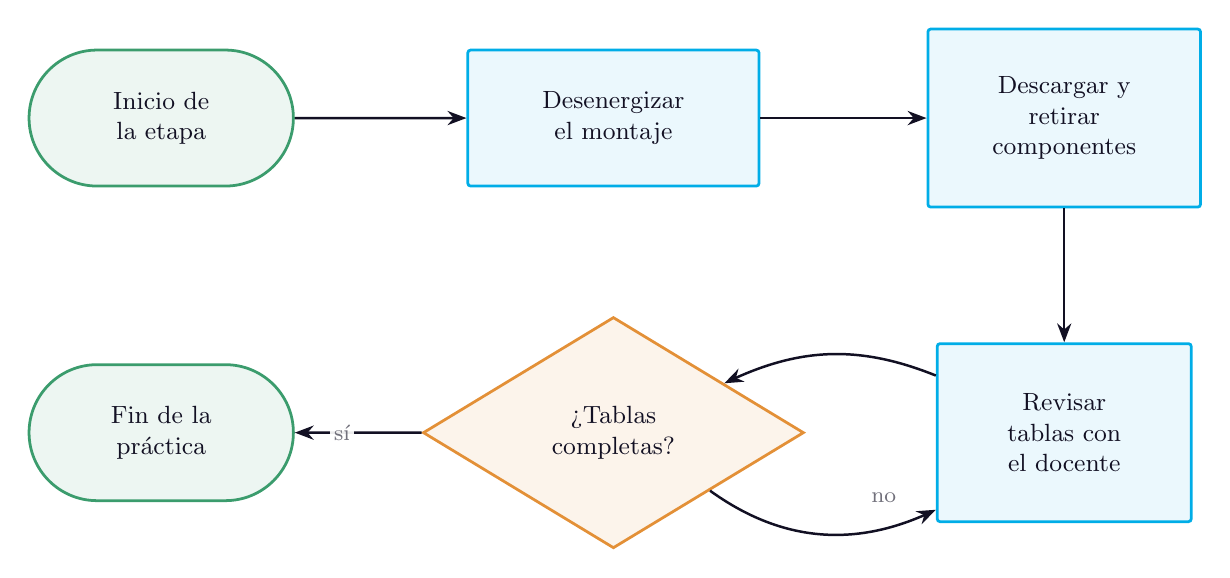
\begin{tikzpicture}[x=1in, y=1in, font=\small]
  % nodos (centro en pulgadas, con el tamano que calcula figuras.py)
  \node[dterminal, minimum width=1.377in, minimum height=0.680in] (n0) at (0.689,-0.445) {Inicio de \\ la etapa};  % ini
  \node[dcaja, minimum width=1.456in, minimum height=0.680in] (n1) at (2.950,-0.445) {Desenergizar \\ el montaje};  % a0
  \node[dcaja, minimum width=1.363in, minimum height=0.890in] (n2) at (5.204,-0.445) {Descargar y \\ retirar \\ componentes};  % a1
  \node[dcaja, minimum width=1.270in, minimum height=0.890in] (n3) at (5.204,-2.018) {Revisar \\ tablas con \\ el docente};  % a2
  \node[ddecision, minimum width=1.905in, minimum height=1.156in] (n4) at (2.950,-2.018) {\textquestiondown{}Tablas \\ completas?};  % dec
  \node[dterminal, minimum width=1.377in, minimum height=0.680in] (n5) at (0.689,-2.018) {Fin de la \\ práctica};  % fin
  % flechas (las de retorno, curvas)
  \draw[dflecha] (n0) -- (n1);
  \draw[dflecha] (n1) -- (n2);
  \draw[dflecha] (n2) -- (n3);
  \draw[dflecha] (n3) to[bend right=24] (n4);
  \draw[dflecha] (n4) -- (n5);
  \draw[dflecha] (n4) to[bend right=31] (n3);
  % rotulos de las flechas (donde no caen sobre un nodo)
  \node[drotulo] at (1.593,-2.018) {sí};
  \node[drotulo] at (4.302,-2.343) {no};
\end{tikzpicture}
\end{adjustbox}
  \caption{Diagrama de flujo de la etapa 4: Desmontaje y cierre}
  \label{fig:flujo-4}
\end{figure}
\begin{pasos}
  \item \textbf{Paso~11:} Apagar el generador de funciones y la fuente, desconectar las puntas del osciloscopio y retirar la alimentación del protoboard. \emph{(aprox.~\SI{3}{\minute})} \textbf{Comprobación:} Ningún indicador de salida debe quedar encendido en el generador ni en la fuente. \textbf{Seguridad:} Desenergizar siempre antes de retirar componentes.
  \item \textbf{Paso~12:} Descargar los condensadores del montaje con la resistencia de descarga, retirar los componentes y devolverlos al kit del grupo con su rótulo. \emph{(aprox.~\SI{4}{\minute})} \textbf{Comprobación:} El kit debe quedar completo, con cada componente en su lugar y con su valor medido anotado.
  \item \textbf{Paso~13:} Revisar con el docente las tablas de registro antes de abandonar el banco. \emph{(aprox.~\SI{3}{\minute})} \textbf{Comprobación:} Las tablas deben estar completas y con unidades; si falta un dato, repetir esa medición antes de desmontar el instrumento.
\end{pasos}

% ---------------------------------------------------------------------
\section{Cuestiones a Resolver}\label{sec:cuestiones}
\begin{enumerate}
  \item \textquestiondown{}Por qué en la resonancia la tensión en el condensador puede ser mayor que la de la fuente?
  \item \textquestiondown{}Qué papel tiene la resistencia de devanado de la bobina en la ley de voltajes de Kirchhoff en la resonancia?
  \item \textquestiondown{}Cómo cambia el carácter del circuito (capacitivo, resistivo o inductivo) al pasar por la resonancia, y cómo se observó?
  \item \textquestiondown{}Qué diferencia hay entre la resonancia medida y la del circuito tanque de la semana 3 con los mismos componentes, y a qué se debe?
\end{enumerate}

% ---------------------------------------------------------------------
\section{Análisis de Resultados}\label{sec:analisis}
Presentar en la tabla de registro la corriente y las tensiones calculadas y medidas a las tres frecuencias, con su diferencia porcentual, y señalar el carácter del circuito en cada una.
\lineablanco
Dibujar el diagrama fasorial de tensiones en la resonancia y a 3 kHz, con la tensión de la bobina real descompuesta en su caída resistiva y su caída reactiva, y comprobar que la suma fasorial reproduce la tensión de la fuente mientras la aritmética no lo hace.
% --- Tabla de registro 1: RLC en serie con VS = 2,00 V eficaces (4 filas vacías para registrar en el banco) ---
\begin{table}[H]
  \centering
  \caption{RLC en serie con VS = 2,00 V eficaces}
  \label{tab:registro-1}
  \arrayrulecolor{iubnavy}
  \begin{tabularx}{\linewidth}{>{\raggedright\arraybackslash}X>{\raggedright\arraybackslash}X>{\raggedright\arraybackslash}X>{\raggedright\arraybackslash}X>{\raggedright\arraybackslash}X>{\raggedright\arraybackslash}X}
    \rowcolor{iubnavy} \textcolor{white}{\textbf{Frecuencia (kHz)}} & \textcolor{white}{\textbf{I (mA)}} & \textcolor{white}{\textbf{VR (V)}} & \textcolor{white}{\textbf{Vbob (V)}} & \textcolor{white}{\textbf{VC (V)}} & \textcolor{white}{\textbf{Carácter}} \\
    \rule{0pt}{0.8cm} & & & & & \\
    \rowcolor{iubfondogris} \rule{0pt}{0.8cm} & & & & & \\
    \rule{0pt}{0.8cm} & & & & & \\
    \rowcolor{iubfondogris} \rule{0pt}{0.8cm} & & & & & \\
    \bottomrule
  \end{tabularx}
\end{table}

% ---------------------------------------------------------------------
\section{Conclusiones}\label{sec:conclusiones}
Concluir si las mediciones reproducen el comportamiento del circuito RLC en serie a ambos lados de la resonancia y en ella, explicando la influencia de la resistencia de devanado y de las capacitancias parásitas; relacionar la práctica con los criterios de medición en circuitos RLC del RA.
\lineablanco
\begin{itemize}
  \item \textquestiondown{}Qué tan cerca estuvo la resonancia medida de la calculada?
  \item \textquestiondown{}Qué demostró la verificación de la ley de voltajes de Kirchhoff en la resonancia?
  \item \textquestiondown{}Qué resultado fue inesperado y cómo se explica?
\end{itemize}

% ---------------------------------------------------------------------
\section{Recomendaciones de Seguridad}\label{sec:seguridad}
\begin{itemize}
  \item Trabajar con el circuito desenergizado mientras se conecta o modifica el montaje; energizar solo después de la revisión del docente.
  \item Mantener la tensión de la fuente en 2,00 V eficaces: en la resonancia en serie la tensión en la bobina y en el condensador supera varias veces la de la fuente \cite{ref1}.
  \item Conectar las tierras de las dos puntas del osciloscopio a un mismo nodo de referencia: unirlas a nodos distintos cortocircuita el elemento que queda entre ellas.
\end{itemize}

% ---------------------------------------------------------------------
\section{Bibliografía}\label{sec:bibliografia}
% Las fuentes cargadas se citan en el texto con \cite{refN}; el \nocite del principio fija su orden y \nocite{*} incluye las demás del .bib.
\nocite{*}
\bibliografia

\end{document}
